\documentclass[fleqn, 11pt]{article}

\usepackage{verbatim}
\usepackage{amsmath}
\DeclareMathOperator*{\argmin}{arg\,min}
\DeclareMathOperator*{\argmax}{arg\,max}
\usepackage{amssymb}
\usepackage{amsthm}
\usepackage{hyperref}
\usepackage{ulem}
\usepackage{enumitem}
\usepackage[left=0.75in, right=0.75in, bottom=0.75in]{geometry}
\usepackage{graphicx}

\newcommand{\myline}{
  \par
  \kern3pt % space above the rules
  \hrule height 0.5pt
  \kern2pt % space between the rules
  \hrule height 0.5pt
  \kern3pt % space below the rules
  \par
}

\usepackage[T1]{fontenc}

\newcommand{\bs}[1]{\boldsymbol{#1}}
\newcommand\norm[1]{\left\lVert#1\right\rVert}

\usepackage{array}
\usepackage{caption}
\usepackage{floatrow}
\usepackage{multirow}

\usepackage{chngcntr}
\counterwithin*{equation}{section}
\counterwithin*{equation}{subsection}

\usepackage{sectsty}
\sectionfont{\centering}

\usepackage[perpage]{footmisc}

\usepackage{fancyhdr}
\pagestyle{fancy}
\fancyhf{}
\lhead{190100036 \& 190100044}
\rhead{CS 754: Assignment 3}
\renewcommand{\footrulewidth}{1.0pt}
\cfoot{Page \thepage}

\setlength{\parindent}{0em}
\renewcommand{\arraystretch}{2}%

\title{CS 754: Advanced Image Processing \\ Project Report}
\author{ 
\begin{tabular}{|c|c|}
     \hline
     \textsf{Krushnakant Bhattad} & \textsf{ \hspace{5pt} Devansh Jain \hspace{5pt} } \\
     \hline
     \textsf{190100036} & \textsf{190100044}\\
     \hline
\end{tabular}
}
\date{May 14, 2021}

\begin{document}

\maketitle
\thispagestyle{empty}
\renewcommand{\arraystretch}{1}%

\myline 

\vspace{7pt}

\underline{\large {\textsc{Project Title}}}: 

\medskip  

Implementing Low-rank matrix completion algorithm for Video denoising and comparing it with other denoising algorithms like PCA and VBM3D method. 

\hrulefill 

\vspace{10pt}

\underline{\large {\textsc{Main Reference Paper}}}: 

\medskip 

"Robust video denoising using low rank matrix completion"

by Hui Ji, Chaoqiang Liu, Zuowei Shen, Yuhong Xu.

Link to the paper: \url{https://ieeexplore.ieee.org/document/5539849}

\hrulefill

\vspace{10pt}

\underline{\large {\textsc{Data set used}}}: 

\medskip 

The original data set can be accessed at: \url{https://media.xiph.org/video/derf/}

\hrulefill

\vspace{10pt}

\underline{\large {\textsc{Validation Strategy}}}: 

\medskip 

We compared our results to that from the methods with impulsive noise pre-processing, like PCA and VBM3D, with respect to their PSNR values (\underline{P}eak \underline{S}ignal to \underline{N}oise \underline{R}atio) and also visually.

\hrulefill

\vspace{10pt}

\underline{\large {\textsc{Associated GitHub Repository}}}:

\medskip

% The working code with results and report is present on the GitHub repository which can accessed at: \url{https://github.com/devansh-dvj/Video-denoising}
The GitHub repository can accessed at: \url{https://github.com/devansh-dvj/Video-denoising/}

\vspace{7pt}

\myline

\newpage
\vspace{-2em}
\myline

\vspace{10pt}

\underline{\large {\textsc{Abstract}}}: 

\medskip  

Most existing video denoising algorithms assume a single statistical model of image noise, e.g. additive Gaussian white noise, which often is violated in practice. The paper presented a new patch-based video denoising algorithm capable of removing serious mixed noise from the video data. \\

The principle is to group similar patches in both spatial and temporal domain to formulate the problem of removing mixed noise as a low-rank matrix completion problem, which leads to a denoising scheme without strong assumptions on the statistical properties of noise. The resulting nuclear norm related minimization problem can be efficiently solved using various techniques, one of which was implemented by us - Singular Value Thresholding algorithm.\\

\vspace{7pt}

\myline 

\vspace{10pt}

\underline{\large {\textsc{Common Abbreviations}}}: 

\medskip  

LRMC - Low Rank Matrix Completion

PCA - Principal Component Analysis

SVD - Singular Value Decomposition

VBM3D - Video block-matching and 3D filtering

\vspace{7pt}

\myline 


\newpage

\section*{The Library}

\subsection*{Adaptive Median Filter (\texttt{adapmedfilt})}

It is step-by-step median filter based on Citation 16 of the Main reference Paper - ``Adaptive median filters: new algorithms and results" by H. Hwang and R. A. Haddad.

\medskip

We consider the first Noise model and use RAMF (ranked-order based adaptive median filter) with a bit of tweaking for computational efficiency.

The filter is based on two level - the first level tests for the presence of residual impulses in the median filter output, and the second level tests whether the center pixel itself is corrupted by an impulse or not.

\medskip

The paper also shows that RAMF is superior to the nonlinear mean $L_1$ filter in removing positive and negative impulses while simultaneously preserving sharpness.

\medskip

Code file: \texttt{libs/adapmedfilt/adapmedfilt.m}

Test file: \texttt{libs/adapmedfilt/adapmedfilt\_test.m}

\bigskip

\subsection*{Noise Model (\texttt{noisemodel})}

In all our experiments, we have taken into account three types of noises - Gaussain, Poission and Impulsive.

\medskip

Gaussian noise (amplifier noise) is zero mean with pixel independent variance $\sigma^2 I$.

Poisson noise (shot noise) is zero mean and variance $\kappa g_k$, where $g_k$ is the pixel intensity.

Impulsive noise by dead pixels, converter or transmission errors and etc with noise level $s$ (in percentage).

\medskip

Code file: \texttt{libs/noisemodel/noisemodel.m}

Test file: \texttt{libs/noisemodel/noisemodel\_test.m}

\bigskip

\subsection*{Patch Matching (\texttt{patchmatcher})}

We use $K$ image frames ($K=50$ by default, but can be varied with experiments).

The patch size is set to $8 \times 8$. 

We sample the reference patches per frame, with a sample interval of 
$4 \times 4$ pixels. 

That means we'd have overlapping patches. 
We also set the range of image intensity to $[0, 255]$.

\medskip

For each reference patch, 5 most similar patches are used in each image frame based on the $\ell_1$ norm distance function.

We use brute force search to find these similar patches. 

Thus, totally $5K$ patches are stacked for the reference patch, and thus the column dimension of the data matrix in the algorithms is $5K$.

\medskip

Code file: \texttt{libs/patchmatcher/patchmatcher.m}

Test file: \texttt{libs/patchmatcher/patchmatcher\_test.m}

\bigskip 

\subsection*{PCA based Denoising (\texttt{pcai})}

Given the $5K$ patches $\{b_q\}_{q=1}^{5K}$, with similar underlying
image structures, we now seek to remove their noise. 

\medskip

Let the
size of each patch be $S \times S = D$. 

We treat each patch $\{b_q\}$ as a
$D$-dimensional vector. 

\medskip

Since all the matched patches have a similar underlying image structure, 
we assume that their noiseless patches lie in a low dimensional subspace, 
centered at $u_0$ and spanned by bases $\{u_d\}_{d=1}^C$. 

\medskip

Let $b'_q$ be the denoised patch for $b_q$: $b'_q = u_0 + \sum_{d=1}^C u_d f_{q,d}$

 where $f_{q,d}$ are the coefficients. 

\medskip

The cost function to be minimised is: $F(\{b'_q\}) = \displaystyle \sum_{q=1}^{5K} \norm{b_q - b'_q}_{\sigma}^2  $

where $\norm{x}_{\sigma}^2 = \displaystyle \sum_{i=1}^D \dfrac{x_i^2}{\sigma_i^2} $ 
is an element-wise variance-normalized
$\ell_2$ norm that accounts for the intensity-dependent noise.

\medskip

The answer to this minimization problem is given by PCA.

\bigskip

We first compute the mean patch $u_0$.

Then, we center the data by subtracting the mean from the input patches. 

Afterward, we normalise each of the $D$ variables by multiplying $i$th element by 
$\sigma_i$ (which is the standard deviation at the $i$th patch pixel). 

\medskip

Then, we apply SVD over on the matrix to obtain the bases, and 
retain the data only along the $C$ 
most ``influential'' dimensions. 

\medskip

We then, de-normalise this data, and add the mean patch 
to each of them to finally get the dimension-reduced data matrix. 

We choose $C$ by trial and error.

\medskip

Code file: \texttt{libs/pcai/pcai.m}

Test file: \texttt{libs/pcai/pcai\_test.m}

\bigskip

\newpage 

\subsection*{LRMC based Denoising (\texttt{svti})}

We form the matrix $P_{j,k}$ using the matched patches. 
The set of missing elements of $P_{j,k}$ has a subset of pixels 
corrupted by impulsive noise using 
the adaptive median filter based impulsive noise detector, while
 
Then, $\Omega$ is formed by including 
the index of all remained pixels. 

\medskip

We solve the problem: \hspace{5pt}
$\min_Q \; ( \dfrac{1}{2} \norm{ Q|_{\Omega} - P|_{\Omega} }_F^2 + \mu \norm{Q}_{*} ) $

\medskip

where $ \norm{Q}_{*} $ is the nuclear norm of $Q$, and $\mu$ is the lagrangian parameter,
which we set according to 

\smallskip

$\mu =  (\sqrt{n_1} + \sqrt{n_2}) \sqrt{p} \hat{\sigma} $. 

\bigskip 

To solve this Low rank matrix completion(LRMC) problem, we use the Fixed point iteration algorithm (Singular Value Thresholding) as described below: 

\bigskip

\includegraphics[scale=0.6]{svt.png}

Here, the shrinkage operator $D_r(X)$ is defined with respect to the Singular Value decomposition $X=U\Sigma V^T$ as $D_r(X)=U\Sigma_r V^T$ (from Candes' paper - Citation 7 of the main reference paper)

The main reference paper implemented another level of search for finding missing pixels using the mean and std. deviation of each row of the matrix. It can be used by setting \texttt{sec\_missing} to true.

\medskip

Code file: \texttt{libs/svti/svti.m}

Test file: \texttt{libs/svti/svti\_test.m}

\begin{comment}
\subsection*{From denoised patches to denoised image}

By applying the two-stage algorithm described above on each patch of input image frames, we can effectively remove most noises from all patches. 

The last step is to synthesize the denoised image from these denoised patches. 

In our implementation, the image patches are sampled with
overlapping regions. Thus, each pixel is covered by several
denoised patches. 

Then, the value of each pixel in images
is determined by taking the average of denoised patches at
this pixel. 

\end{comment}

\newpage

\section*{The Algorithms (\texttt{LRMC} and \texttt{PCA})}

Given an input noisy image sequence $\{\mathcal{I}\}_{i=1}^{K}$, 
we first apply
the adaptive median filter to the images, so as to 
identify the pixels corrupted by impulsive
noise and replace those damaged pixels by the median of 
small neighborhood.

\medskip

Next, we create 
a patch-Array, where:

The patch size is set to $8 \times 8$, and 

We sample the reference patches per frame, with a sample interval of 
$4 \times 4$ pixels. 

\bigskip 

De-noising a patch:

\smallskip

Given this patch-Array, we do Patch Matching to obtain a stack of $5K$ 
most similar patches. 

Then, we apply the LRMC-based or PCA-based denoising on
this stack of patches, to obtain denoised patch.

\medskip

Doing this for each patch, 
we can effectively remove most noise from all patches. 

\bigskip

The last step is to synthesize the denoised images from these denoised patches.

\medskip

In our implementation, the image patches are sampled with
overlapping regions. Thus, each pixel is covered by several
denoised patches. 

\medskip

Then, the value of each pixel in images
is determined by taking the average of denoised patches at
this pixel. 

\medskip

This gives us the final denoised images.

\bigskip
\bigskip

LRMC Algorithm has four variants based on whether while iterating we update the patch array and whether we should consider second subset of missing pixels in \texttt{svti}

\medskip

PCA Algorithm has two variants based on whether while iterating we update the patch array or not.

\bigskip

Code file for LRMC: \texttt{algos/LRMC/LRMC.m}

Code file for PCA: \texttt{algos/PCA/PCA.m}


\newpage 

\section*{The Results}

\subsection*{Comparing Algorithms}

\begin{itemize}[noitemsep]
    \item \texttt{LRMC1} : Low Rank Matrix Completion Algorithm with variant `01', $\tau = 1.5$, k$_\text{max}$ 30, tol 1e-5
    \item \texttt{LRMC2} : Low Rank Matrix Completion Algorithm with variant `10', $\tau = 1.5$, k$_\text{max}$ 30, tol 1e-5
    \item \texttt{PCA1} : Principal Component Analysis Algorithm with variant `0', C = 2
    \item \texttt{PCA2} : Principal Component Analysis Algorithm with variant `0', C = 4
    \item \texttt{PCA3} : Principal Component Analysis Algorithm with variant `0', C = 8
    \item \texttt{PCA4} : Principal Component Analysis Algorithm with variant `0', C = 16
    \item \texttt{VBM3D1} : VBM3D Algorithm with the adaptive median filter applied to the noisy video
    \item \texttt{VBM3D2} : VBM3D Algorithm without the adaptive median filter
\end{itemize}

\begin{table}[H]
    \centering
    \begin{tabular}{||c|c||c|c||c|c|c|c||c|c||}
         \hline
         \multirow{2}{*}{\{$\sigma$, $\kappa$\}} & \multirow{2}{*}{$s$} & \multicolumn{8}{c||}{PSNR of Reconstructed Frames} \\
         \cline{3-10}
         & & LRMC1 & LRMC2 & PCA1 & PCA2 & PCA3 & PCA4 & VBM3D1 & VBM3D2 \\
         \hline
         \multirow{5}{*}{\{10, 10\}} & 10\% & 23.6945 & 23.5994 & 27.1342 & 27.3721 & 27.2584 & 26.4753 & 23.7962 & 17.5443 \\
         \cline{2-10}
          & 20\% & 23.1713 & 23.1008 & 26.6927 & 26.8437 & 26.6462 & 25.8998 & 23.1268 & 15.5175 \\
         \cline{2-10}
          & 30\% & 22.6781 & 22.5920 & 26.1415 & 26.2657 & 26.0366 & 25.2296 & 22.5524 & 14.1236 \\
         \cline{2-10}
          & 40\% & 22.2009 & 22.1286 & 25.5636 & 25.5995 & 25.3423 & 24.4537 & 21.9991 & 13.0405 \\
         \cline{2-10}
          & 50\% & 21.8527 & 21.7505 & 24.9397 & 24.9599 & 24.6227 & 23.6796 & 21.6151 & 12.2634 \\
         \hline
         \multirow{3}{*}{\{50, 5\}} & 10\% & 21.9801 & 22.0652 & 25.2479 & 25.2414 & 24.9745 & 24.2019 & 27.3927 & 23.9866 \\
         \cline{2-10}
          & 30\% & 21.3173 & 21.3527 & 24.4847 & 24.4564 & 24.1792 & 23.3586 & 26.3149 & 17.0644 \\
         \cline{2-10}
          & 50\% & 20.5023 & 20.4782 & 23.4038 & 23.2987 & 22.9143 & 21.9643 & 24.9581 & 14.3543 \\
         \hline
    \end{tabular}
\end{table}

\vspace{-2em}
\begin{figure}[H]
    \centering
    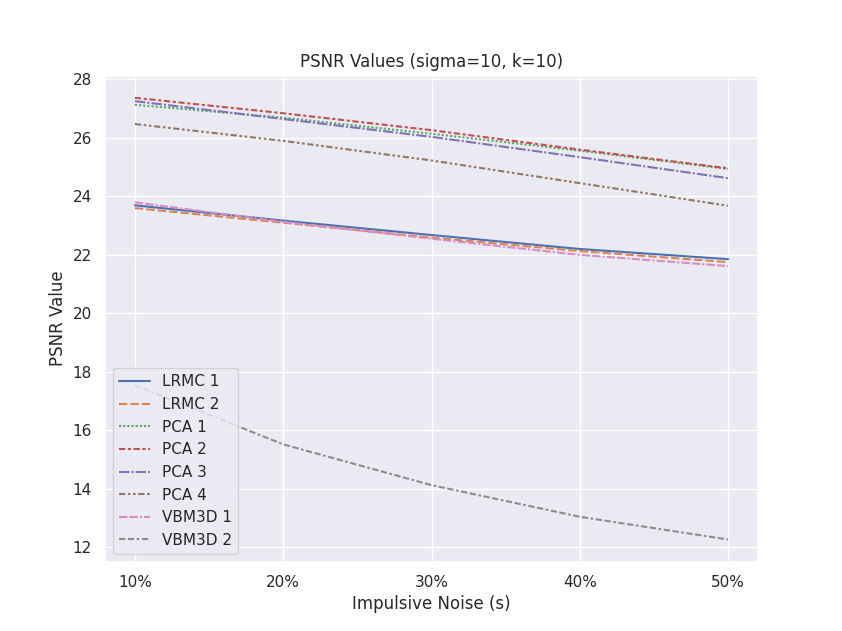
\includegraphics[scale=0.7]{sigma10k10.png}
\end{figure}

\begin{figure}[H]
    \centering
    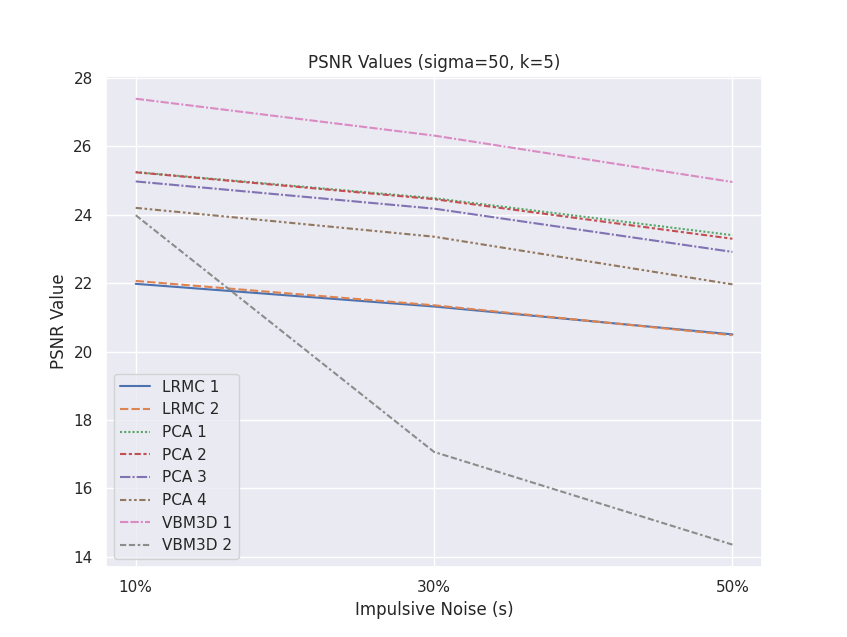
\includegraphics[scale=0.7]{sigma50k5.png}
\end{figure}

\textbf{Inferences}:

\begin{itemize}
    \item $\sigma = 10$, $\kappa = 10$ means low Gaussian and moderate Poisson noise. Here, PCA outperforms both LRMC and VBM3D by large margins, and LMRC performs almost on par with VBM3D+Adaptive Median Filter; moreover LRMC starts overtakes VBM3D+Adaptive Median Filter as impulsive noise increases.   
    
    \item $\sigma = 50$, $\kappa = 5$ means high Gaussian and low Poisson noise. Since VBM3D's noise model is based on additive white gaussian noise, here VBM3D (with median filtering to remove impulsive noise) performs better than both LRMC and PCA methods.
    
    \item In any case, as impulsive noise increases, VBM3D's performance decreases more steeply than PCA or LRMC. 
    
    \item Without adaptive median filtering (which is an integral part of our method), VBM3D fails to perform in almost all cases, as especially seen when there is high impulsive noise.
\end{itemize}

\newpage
\subsection*{Comparing effects of change of parameters in LRMC}

We work on $\sigma = 10$, $\kappa = 10$ and $s = 30\%$ for the following LRMC runs.

k$_\text{max}$ is maximum number of iterations .

\begin{table}[H]
    \centering
    \begin{tabular}{||c|c|c||c|c|c|c||}
         \hline
         \multirow{2}{*}{tol} & \multirow{2}{*}{$\tau$} & \multirow{2}{*}{k$_\text{max}$} & \multicolumn{4}{c||}{PSNR of Reconstructed Frames} \\
         \cline{4-7}
         & & & Variant `00' & Variant `01' & Variant `10' & Variant `11' \\
         \hline
         \multirow{6}{*}{1e-5} & \multirow{2}{*}{1.0} & 30 & 21.6253 & 21.6466 & 21.4761 & 21.4979 \\
         \cline{3-7}
          & & 60 & 21.8325 & 21.8561 & 21.6951 & 21.7238 \\
         \cline{3-7}
          & \multirow{2}{*}{1.5} & 30 & 21.8286 & 21.8527 & 21.6910 & 21.7201 \\
         \cline{3-7}
          & & 60 & 21.8327 & 21.8562 & 21.6952 & 21.7241 \\
         \cline{3-7}
          & \multirow{2}{*}{2.0} & 30 & 21.8325 & 21.8560 & 21.6951 & 21.7239 \\
         \cline{3-7}
          & & 60 & 21.8327 & 21.8562 & 21.6952 & 21.7241 \\
         \hline
    \end{tabular}
\end{table}

\begin{figure}[H]
    \centering
    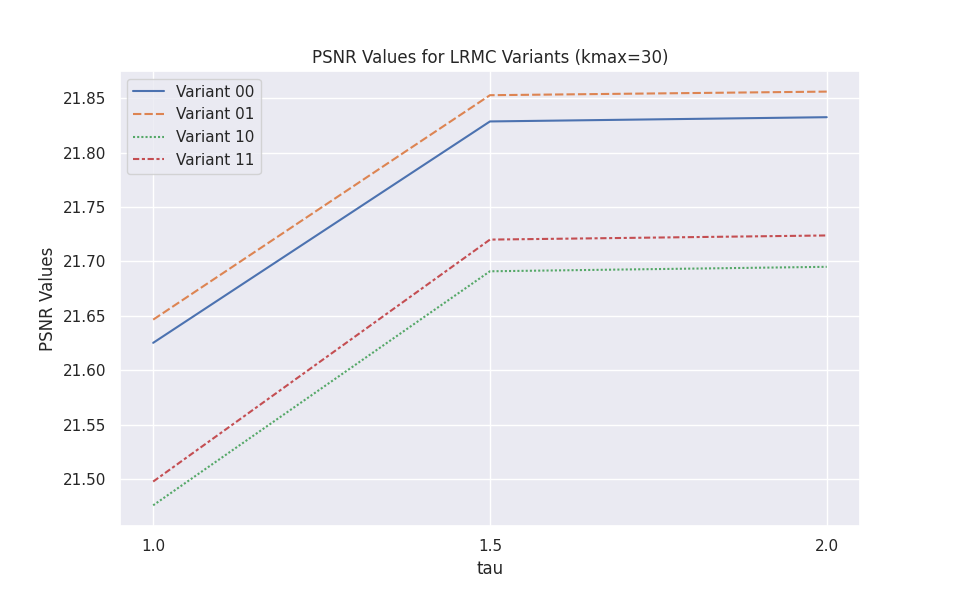
\includegraphics[scale=0.7]{kmax=30.png}
\end{figure}

\begin{figure}[H]
    \centering
    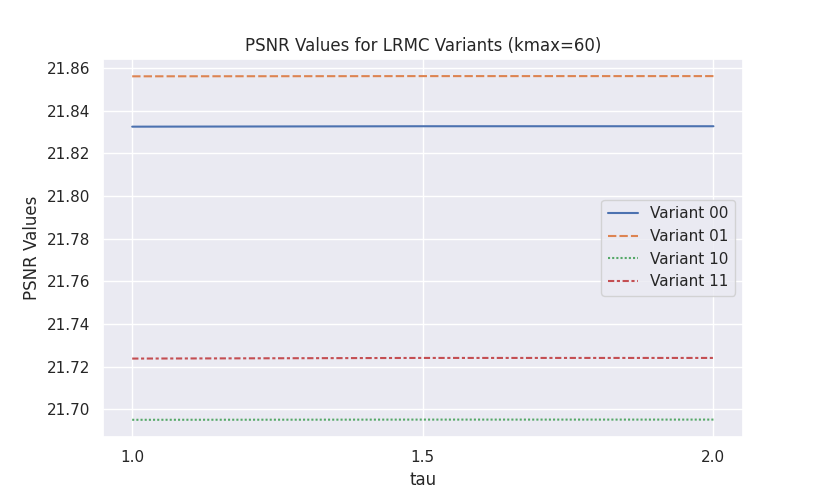
\includegraphics[scale=0.8]{kmax=60.png}
\end{figure}

\textbf{Inferences}:

\begin{itemize}
    \item $\tau$ denotes the step-size. It has been observed that for $\tau \in [1, 2]$, SVT algorithm converges.
    \item For bigger step-size, i.e. for $\tau = 2$, we reach to convergence faster with less number of iterations for reaching the tolerance limit, with k$_\text{max} = 30$ giving satisfactory results.
    \item For smaller step-size, i.e. for $\tau = 1$, we reach to convergence slower with more number of iterations for reaching the tolerance limit, wit k$_\text{max} = 30$ giving relative lower PSNR values. So, we require k$_\text{max} = 60$ to reach satisfactory results.
    \item Also, comparing the variants, we can see that `01' gives the best results followed by `00', `11', `10', i.e. iteratively updating patch array gives better results but including second subset of missing pixels doesn't.
\end{itemize}

\newpage
\subsection*{Comparing Reconstructed Images visually}

\textbf{$\sigma = 10$, $\kappa = 10$, $s = 30\%$}
\begin{figure}[H]
    \centering
    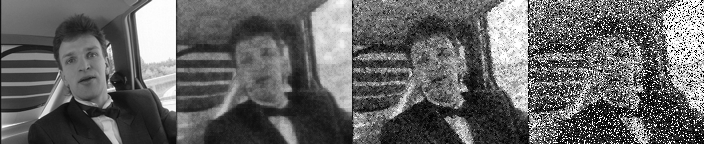
\includegraphics[scale=0.7]{10_10_30_LRMC1.png}
    \caption{\texttt{LRMC1}, left to right - original, reconstructed, filtered, noisy frame}
\end{figure}
\begin{figure}[H]
    \centering
    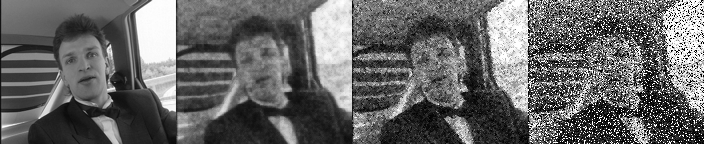
\includegraphics[scale=0.7]{10_10_30_PCA2.png}
    \caption{\texttt{PCA2}, left to right - original, reconstructed, filtered, noisy frame}
\end{figure}
\begin{figure}[H]
    \centering
    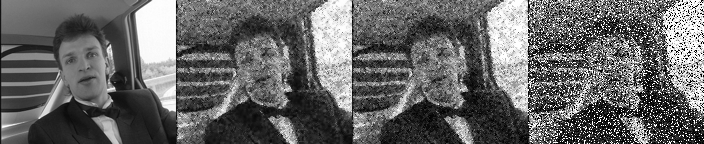
\includegraphics[scale=0.7]{10_10_30_VBM3D1.png}
    \caption{\texttt{VBM3D1}, left to right - original, reconstructed, filtered, noisy frame}
\end{figure}
\begin{figure}[H]
    \centering
    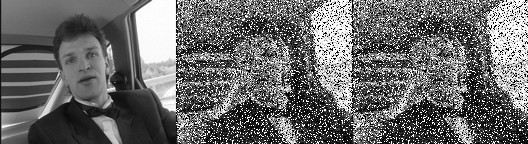
\includegraphics[scale=0.7]{10_10_30_VBM3D2.png}
    \caption{\texttt{VBM3D2}, left to right - original, reconstructed, noisy frame}
\end{figure}

\newpage
\textbf{$\sigma = 10$, $\kappa = 10$, $s = 50\%$}
\begin{figure}[H]
    \centering
    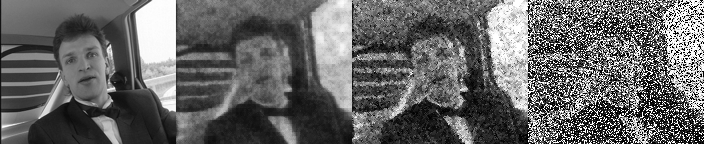
\includegraphics[scale=0.7]{10_10_50_LRMC1.png}
    \caption{\texttt{LRMC1}, left to right - original, reconstructed, filtered, noisy frame}
\end{figure}
\begin{figure}[H]
    \centering
    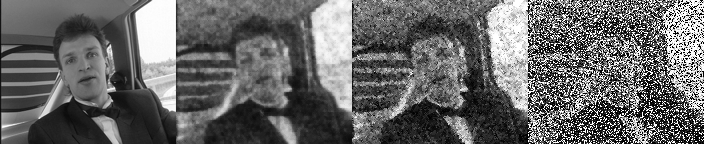
\includegraphics[scale=0.7]{10_10_50_PCA2.png}
    \caption{\texttt{PCA2}, left to right - original, reconstructed, filtered, noisy frame}
\end{figure}
\begin{figure}[H]
    \centering
    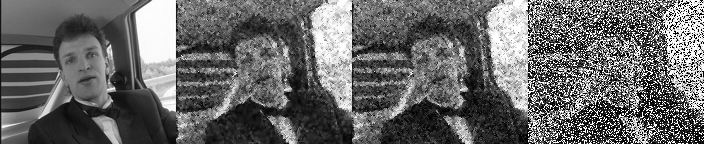
\includegraphics[scale=0.7]{10_10_50_VBM3D1.png}
    \caption{\texttt{VBM3D1}, left to right - original, reconstructed, filtered, noisy frame}
\end{figure}
\begin{figure}[H]
    \centering
    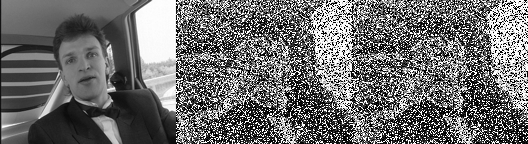
\includegraphics[scale=0.7]{10_10_50_VBM3D2.png}
    \caption{\texttt{VBM3D2}, left to right - original, reconstructed, noisy frame}
\end{figure}

\newpage
\textbf{Inferences}:

\begin{itemize}
    \item Clearly, VBM3D without filtering doesn't make significant change to the noisy image and thus, is not a good denoiser for impulsive noise.
  
    \item Even if we add filtering before VBM3D, we can still see a lot of impulsive pixels distinctly visible.
  
    \item PCA2 gave the best PSNR of all PCAs and had better PSNR than both LRMC and VBM3D but it over-smoothens the image. Also, we don't know the appropriate value of C. For best results, we would have to use something like binary search.
  
    \item LRMC does a nice job removing the hazziness caused due to impulsive noise, even though it does add a bit of blurring due to low rank matrix completion run considering the impulsive pixels as missing pixels and gaussian and poisson blurring is carried to those pixels.
    
    \item LRMC algorithm does not use existing impulsive noise remover (adaptive median filter) to remove impulsive noise. Instead, it uses the existing impulsive noise detector to detect those damaged (missing) pixels which are further refined by a census along the row in the matched patch stack.
\end{itemize}

\end{document}

